\documentclass{standalone}

\usepackage{tikz}
\usepackage{circuitikz}

\tikzset{block/.style = {draw, fill=white, very thick, rectangle, minimum height=1cm, minimum width=2cm},
         lblock/.style={draw,fill=white,very thick, rectangle, minimum height=3cm, minimum width=1cm},
         sum/.style= {draw, fill=white, very thick, circle, node distance=0.5cm}}

         
\begin{document}
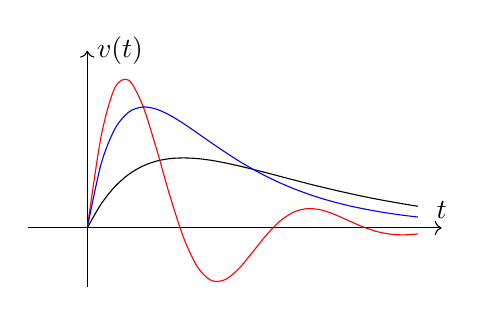
\begin{tikzpicture}[scale=1.5]
    \draw[->](-0.5,0)--(3,0)node[above]{$t$};
    \draw[->](0,-0.5)--(0,1.5)node[right]{$v(t)$};

    \draw[black]plot[smooth, domain=0:2.8](\x,{-4*e^(-1.5*\x)+4*e^(-\x)});        
    \draw[red]plot[smooth, domain=0:2.8](\x,{2*e^(-1.3*\x)*sin(4*\x r)});
    \draw[blue]plot[smooth, domain=0:2.8](\x,{-e^(-4*\x)+3*\x*e^(-2*\x)+e^(-\x)});
\end{tikzpicture}
\end{document}